\documentclass[tikz]{standalone}
\usepackage{fontspec}
\renewcommand*{\familydefault}{\sfdefault}
\usepackage{standalone}
\usetikzlibrary{arrows.meta, decorations.pathreplacing, shapes.geometric}
%\usetikzlibrary{positioning,fit,shapes.geometric,fadings,bayesnet}

\begin{document}

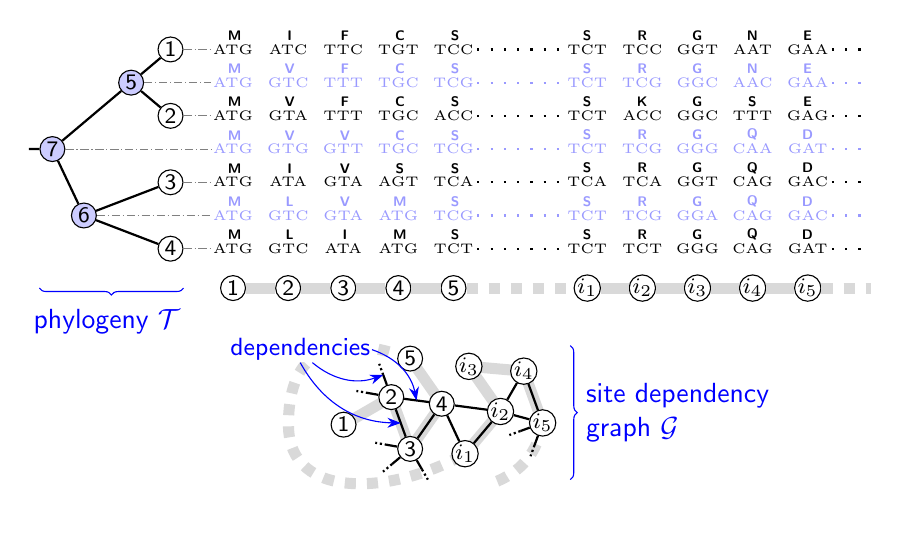
\begin{tikzpicture} 
[font=\tiny, label distance=0 cm, inner sep=0.5 pt,
every node/.style={anchor=center},
%every label/.style={blue},
itc/.style={blue!40!white, font={\rmfamily\tiny}},
otc/.style={black, font={\rmfamily\tiny}},
ita/.style={blue!40!white, font={\bfseries\tiny}},
ota/.style={black, font={\bfseries\tiny}},
]

% first block of alignment
\matrix[column sep={0.7 cm,between origins}, row sep={12 pt,between origins}] (codon-aln) at (0,0) {
\node[otc] (v1) {ATG}; & \node[otc] {ATC}; & \node[otc] {TTC}; & \node[otc] {TGT}; & \node[otc] {TCC}; \\
\node[itc] (v5) {ATG}; & \node[itc] {GTC}; & \node[itc] {TTT}; & \node[itc] {TGC}; & \node[itc] {TCG}; \\
\node[otc] (v2) {ATG}; & \node[otc] {GTA}; & \node[otc] {TTT}; & \node[otc] {TGC}; & \node[otc] {ACC}; \\
\node[itc] (v7) {ATG}; & \node[itc] {GTG}; & \node[itc] {GTT}; & \node[itc] {TGC}; & \node[itc] {TCG}; \\
\node[otc] (v3) {ATG}; & \node[otc] {ATA}; & \node[otc] {GTA}; & \node[otc] {AGT}; & \node[otc] {TCA}; \\
\node[itc] (v6) {ATG}; & \node[itc] {GTC}; & \node[itc] {GTA}; & \node[itc] {ATG}; & \node[itc] {TCG}; \\
\node[otc] (v4) {ATG}; & \node[otc] (s2) {GTC}; & \node[otc] (s3) {ATA}; & \node[otc] (s4) {ATG}; & \node[otc] (s5) {TCT}; \\ };
\matrix[column sep={0.7 cm,between origins}, row sep={12 pt,between origins}] (aa-aln) at (0,5 pt) {
\node[ota] (u1)  {M} ; & \node[ota]  {I} ; & \node[ota]  {F} ; & \node[ota]  {C} ; & \node[ota]  {S} ; \\
\node[ita] (u5)  {M} ; & \node[ita]  {V} ; & \node[ita]  {F} ; & \node[ita]  {C} ; & \node[ita]  {S} ; \\
\node[ota] (u2)  {M} ; & \node[ota]  {V} ; & \node[ota]  {F} ; & \node[ota]  {C} ; & \node[ota]  {S} ; \\
\node[ita] (u7)  {M} ; & \node[ita]  {V} ; & \node[ita]  {V} ; & \node[ita]  {C} ; & \node[ita]  {S} ; \\
\node[ota] (u3)  {M} ; & \node[ota]  {I} ; & \node[ota]  {V} ; & \node[ota]  {S} ; & \node[ota]  {S} ; \\
\node[ita] (u6)  {M} ; & \node[ita]  {L} ; & \node[ita]  {V} ; & \node[ita]  {M} ; & \node[ita]  {S} ; \\
\node[ota] (u4)  {M} ; & \node[ota]  {L} ; & \node[ota]  {I} ; & \node[ota]  {M} ; & \node[ota]  {S} ; \\ };

% second block of alignment
\matrix[column sep={0.7 cm,between origins}, row sep={12 pt,between origins}] (codon-aln-2) at (4.5 cm,0) {
\node[otc] (w1) {TCT}; & \node[otc] {TCC}; & \node[otc] {GGT}; & \node[otc] {AAT}; & \node[otc] {GAA}; \\
\node[itc] (w5) {TCT}; & \node[itc] {TCG}; & \node[itc] {GGC}; & \node[itc] {AAC}; & \node[itc] {GAA}; \\
\node[otc] (w2) {TCT}; & \node[otc] {ACC}; & \node[otc] {GGC}; & \node[otc] {TTT}; & \node[otc] {GAG}; \\
\node[itc] (w7) {TCT}; & \node[itc] {TCG}; & \node[itc] {GGG}; & \node[itc] {CAA}; & \node[itc] {GAT}; \\
\node[otc] (w3) {TCA}; & \node[otc] {TCA}; & \node[otc] {GGT}; & \node[otc] {CAG}; & \node[otc] {GAC}; \\
\node[itc] (w6) {TCT}; & \node[itc] {TCG}; & \node[itc] {GGA}; & \node[itc] {CAG}; & \node[itc] {GAC}; \\
\node[otc] (w4) {TCT}; & \node[otc] (s7) {TCT}; & \node[otc] (s8) {GGG}; & \node[otc] (s9) {CAG}; & \node[otc] (s10) {GAT}; \\ };
\matrix[column sep={0.7 cm,between origins}, row sep={12 pt,between origins}] (aa-aln-2) at (4.5 cm,5 pt) {
\node[ota] (x1)  {S} ; &  \node[ota] {R} ; & \node[ota]  {G} ; & \node[ota]  {N} ; & \node[ota]  {E} ; \\
\node[ita] (x5)  {S} ; &  \node[ita] {R} ; & \node[ita]  {G} ; & \node[ita]  {N} ; & \node[ita]  {E} ; \\
\node[ota] (x2)  {S} ; &  \node[ota] {K} ; & \node[ota]  {G} ; & \node[ota]  {S} ; & \node[ota]  {E} ; \\
\node[ita] (x7)  {S} ; &  \node[ita] {R} ; & \node[ita]  {G} ; & \node[ita]  {Q} ; & \node[ita]  {D} ; \\
\node[ota] (x3)  {S} ; &  \node[ota] {R} ; & \node[ota]  {G} ; & \node[ota]  {Q} ; & \node[ota]  {D} ; \\
\node[ita] (x6)  {S} ; &  \node[ita] {R} ; & \node[ita]  {G} ; & \node[ita]  {Q} ; & \node[ita]  {D} ; \\
\node[ota] (x4)  {S} ; &  \node[ota] {R} ; & \node[ota]  {G} ; & \node[ota]  {Q} ; & \node[ota]  {D} ; \\ };

% dotted lines after first block
\draw[thick, loosely dotted]
foreach \x in {1,...,4}
{
(codon-aln.east|-w\x) -- (codon-aln-2.west|-w\x)
(codon-aln-2.east|-w\x) -- +(0.5,0)
}
;

% dotted lines after second block
\draw[thick, loosely dotted, blue!40!white]
foreach \x in {5,...,7}
{
(codon-aln.east|-w\x) -- (codon-aln-2.west|-w\x)
(codon-aln-2.east|-w\x) -- +(0.5,0) coordinate (s11)
}
;

\begin{scope}[font={\footnotesize}, every node/.style={draw, inner sep=0 pt, minimum size=9 pt,
circle, fill=white}]

% nodes of phylogeny
\path[draw]
foreach \x in {1,...,4}
{(v\x-|codon-aln.west) +(-0.5,0) node (V\x) {\x}}
(v5-|codon-aln.west) +(-1,0) node[fill=blue!20!white] (V5) {5}
(v6-|codon-aln.west) +(-1.6,0) node[fill=blue!20!white] (V6) {6}
(v7-|codon-aln.west) +(-2.0,0) node[fill=blue!20!white] (V7) {7}
;

% draw phylogeny
\draw[thick]
(V7) -- (V5)
(V5) -- (V1)
(V5) -- (V2)
(V7) -- (V6)
(V6) -- (V3)
(V6) -- (V4)
(V7) -- +(-0.3,0)
;
\draw[thin, gray, densely dash dot]
foreach \x in {1,...,7}
{(V\x) -- (v\x)}
;

% site nodes to the bottom of columns
\path[draw]
(v4) coordinate (s1)
(w4) coordinate (s6)
foreach \x in {1,...,5}
{(s\x) +(0,-0.5) node (S\x) {\x}}
foreach \x/\y in {6/1,7/2,8/3,9/4,10/5}
{(s\x) +(0,-0.5) node (S\x) {\(i_\y\)}}
(S10-|s11) coordinate (S11)
;

% peptide backbone
\draw[line width=4 pt, gray!30!white]
(S1) -- (S2)
(S2) -- (S3)
(S3) -- (S4)
(S4) -- (S5)
(S6) -- (S7)
(S7) -- (S8)
(S8) -- (S9)
(S9) -- (S10)
;
\draw[line width=4 pt, gray!30!white, loosely dotted]
(S5) -- (S6)
(S10) -- (S11)
;


% SCHEMATI STRUCTURE
\begin{scope}[yshift=-3.5 cm]

% position sites in schematic structure
\draw[line width=4 pt, gray!30!white]
(0,0) coordinate (a1)
-- ++(30:0.7) coordinate (a2)
-- ++(-70:0.7) coordinate (a3)
-- ++(55:0.7) coordinate (a4)
-- ++(125:0.7) coordinate (a5)
(a3) ++(-5:0.7) coordinate (a6)
-- ++(50:0.7) coordinate (a7)
-- ++(125:0.7) coordinate (a8)
-- ++(-05:0.7) coordinate (a9)
-- ++(-70:0.7) coordinate (a10)
;

% dashed peptide backbone
\draw[line width=4 pt, gray!30!white, loosely dotted]
(a5) .. controls ++(160:1) and ++(90:1) .. (-0.7,0)
.. controls ++(-90:1) and ++(210:1) .. (a6)
(a10) to[bend left] ++(-130:1.0)
;

% site labels
\path[draw] foreach \x in {1,...,5}
{(a\x) node (A\x) {\x}}
;
\path[draw] foreach \x/\y in {6/1,7/2,8/3,9/4,10/5}
{(a\x) node (A\x) {\(i_\y\)}}
;

% site dependencies
\draw[thick]
(A2) -- coordinate (A2A3) (A3)
(A2) -- coordinate (A2A4) (A4)
(A3) -- (A4)
(A4) -- (A6)
(A4) -- (A7)
(A6) -- (A7)
(A7) -- (A9)
(A7) -- (A10)
(A9) -- (A10)
;

\path
(A2) ++(110:0.3 cm) coordinate (B2a) ++(110:0.15 cm) coordinate (C2a)
(A2) ++(170:0.3 cm) coordinate (B2b) ++(170:0.15 cm) coordinate (C2b)
(A3) ++(220:0.3 cm) coordinate (B3a) ++(220:0.15 cm) coordinate (C3a)
(A3) ++(170:0.3 cm) coordinate (B3b) ++(170:0.15 cm) coordinate (C3b)
(A3) ++(-60:0.3 cm) coordinate (B3c) ++(-60:0.15 cm) coordinate (C3c)
%(A9) ++(220:0.3 cm) coordinate (B9a) ++(220:0.15 cm) coordinate (C9a)
(A10) ++(250:0.3 cm) coordinate (B10a) ++(250:0.15 cm) coordinate (C10a)
(A10) ++(200:0.3 cm) coordinate (B10b) ++(200:0.15 cm) coordinate (C10b)
;

\draw[thick]
(A2) -- (B2a)
(A2) -- (B2b)
(A3) -- (B3a)
(A3) -- (B3b)
(A3) -- (B3c)
(A10) -- (B10a)
(A10) -- (B10b)
;

\draw[thick, densely dotted]
(B2a) -- (C2a)
(B2b) -- (C2b)
(B3a) -- (C3a)
(B3b) -- (C3b)
(B3c) -- (C3c)
(B10a) -- (C10a)
(B10b) -- (C10b)
;

\end{scope}
\end{scope}

% point at dependencies
\begin{scope}[blue, font=\normalsize]

\begin{scope}[->, arrows = {-Stealth}]
\path (A1) +(120:1.1) node[fill=white, shape=rectangle, font={\small}] (A0) {dependencies};
%\path (120:1.1) node[shape=rectangle] (A0) {dependencies};
\draw (A0.south) to[bend right] (A2A3);
\draw (A0.east) to[bend left] (A2A4) ;
\draw (A0) to[bend right] (B2a) ;
\end{scope}

\draw[decorate, decoration={brace, mirror}]
(V7.west|-S1) --
node[below=7 pt, align=center] {phylogeny \(\mathcal{T}\) }
(V1.east|-S1)
;

% label for site dependency graph
\draw[decorate, decoration={brace, raise=10 pt}]
(A10|-A5.north) --
node[right=15 pt, align=left] {site dependency\\graph \(\mathcal{G}\)}
(A10|-C3c)
;

\end{scope}

\end{tikzpicture}
\end{document}
